%% Le lingue utilizzate, che verranno passate come opzioni al pacchetto babel. Come sempre, l'ultima indicata sarà quella primaria.
%% Se si utilizzano una o più lingue diverse da "italian" o "english", leggere le istruzioni in fondo.
\def\thudbabelopt{italian,english}
%% Valori ammessi per target: bach (tesi triennale), mst (tesi magistrale), phd (tesi di dottorato).
%% --- Beamer ---
%% La chiave "beamer" attiva la modalità slide e specifica le opzioni da passare all'omonima classe.
%% Le opzioni specificate "noamsthm,10pt" sono solamente indicative.
%% L'uso dell'opzione "ignorenonframetext" può creare problemi ed è quindi sconsigliato.
%% Se incontrate problemi con altre opzioni di "beamer" fatecelo sapere.
%\documentclass{beamer}
\documentclass[beamer={noamsthm,10pt},target=bach]{thud}[2014/03/11]
\usetheme{uniud}

\usepackage{tikz}
\usepackage{verbatim, fancyvrb}
\usepackage{multirow}
\usepackage{array}
%% --- Informazioni sulla tesi ---
%% Per tutti i tipi di tesi
\title{Implementation of Open Transactional Memory in Haskell}
\author{Valentino Picotti}
\course{Informatica}
\supervisor{Prof.\ Marino Miculan}
\cosupervisor{Marco Peressotti\and Nicola Gigante}
%% Altri campi disponibili: \tutor, \date (anno accademico, calcolato in automatico).
%% Con \supervisor, \cosupervisor e \tutor si possono indicare più nomi separati da \and.
%% Per le sole tesi di dottorato
%\cycle{XXVIII}
%% Campi obbligatori: \title, \author e \course.

%% Nel resto del preambolo potete personalizzare la presentazione liberamente.
%% Se incontrate problemi causati dall'interazione tra "thud" e "beamer" fatecelo sapere.
\usetikzlibrary{calc,arrows}
\tikzset{
      nodesr/.style={
          rectangle,
          thick,
          draw=black,
          minimum size=4mm
      }
  }

\begin{document}

%% Il frontespizio prima di tutto!
%% \maketitle accetta gli stessi argomenti opzionali di \begin{frame} (p.es. "[plain]")
\maketitle

%% Sezione
\section{Introduction}

% \begin{frame}{Multi-threaded Programming}
% The advent of multi-core architectures crucial write correct and scalable multi-threaded programs
% \end{frame}
%% Diapositiva
%\subsection{Transactional Memory}
\begin{frame}{Transactional Memory}
%The advent of multi-core architectures 

% In multi-threaded programs, threads can interact through shared memory.

\emph{Transactional Memory} (TM) has emerged as a promising alternative to traditional \emph{lock-based} synchronization.

Blocks of code are marked as \emph{atomic} and their execution will appear either if it was performed instantaneously at some unique point in time, or, if aborted, as if it never happened.
% Advantages of TM:
% \begin{itemize}
% \item Lock-free programming
% \item Avoids deadlocks, race conditions and priority inversions
% \item Composability and scalability
% \item Exploit multi-core architectures
% \end{itemize}
\end{frame}

%% Sottosezione
%\subsection{Sottosezione}
% \begin{frame}{Transactional Memory: the idea}

% \end{frame}

%\subsection{The problem}

\begin{frame}[fragile]{The problem with interacting transactions}
Most TM models admit only \emph{isolated} transactions, which are not adequate in multi-threaded programming where transactions have to interact via shared data \emph{before} committing.

A simple example is a request-response interaction via a shared buffer. Synchronization is required to regulate accesses to the buffer.

\begin{figure}
\centering
\begin{minipage}[t]{0.5\textwidth}
\begin{BVerbatim}[baseline=t]
// Party1 (Master)
atomically {
  // put request in b
  up(c1);
  // some other code
  down(c2);
  // get answer from b
}
\end{BVerbatim}
\end{minipage}
\begin{minipage}[t]{0.4\textwidth}
\begin{BVerbatim}[baseline=t]
// Party2 (Worker)
atomically {
  // some code before
  down(c1);
  // get request from b
  // put answer in b
  up(c2);
  // some code after
}
\end{BVerbatim}
\end{minipage}
\end{figure}
\end{frame}

% \begin{frame}[fragile]{Example}

% \note{Any admissible execution requires an interleaved scheduling between the two transactions, thus violating isolation}
% \note{Deadlock arises only because we are inside isolated transactions, the solution above is fine for threads outside transactions or within the same transaction}
% \end{frame}

%\subsection{Thesis proposal}
% \begin{frame}{Thesis proposal}
% The key observation is that \emph{atomicity} and \emph{isolation} should be seen as two disjoint computational aspects.

% \begin{itemize}
% \item<2->{an atomic \emph{non-isolated} block is executed ``all-or-nothing''}
% \note{but its execution can overlap that of others and uncontrolled acces to shared data is allowed}
% \item<3->{an \emph{isolated} block of code is executed ``as it were the only one''}
% \end{itemize}
% \end{frame}

% \begin{frame}[fragile]{Open transactions}
% Atomic non-isolated blocks can be used for implementing safe composable interacting memory transactions, called \emph{open transactions}.


% \begin{figure}
% \centering

% \begin{tabular}{ c | c | c |}
% \cline{2-3}
% & non-atomic & atomic \\
% \hline
% \multicolumn{1}{|c|}{isolated} & mutex block & TM\\
% \hline
% \multicolumn{1}{|c|}{non-isolated} & Normal block & Open transactions\\
% \hline
% \end{tabular}
% \end{figure}

% \end{frame}

\section{OTM}

\begin{frame}{OTM}
\emph{Open Transactional Memory} (OTM) is the model that implements \emph{open transactions}. In this model:%\onslide<2->{In this model:}
\begin{itemize}
\item%<2->
a transaction is composed by several threads, called \emph{participants}
\item%<3->
a transaction commits when all its participants commit, and aborts if any thread aborts
\item%<4->
accesses to shared data cause transactions to be \emph{transparently merged} into a single one
\end{itemize}

\begin{figure}
\centering
\begin{tabular}{ c | c | c |}
\cline{2-3}
& non-atomic & atomic \\
\hline
\multicolumn{1}{|c|}{non-isolated} & Normal block & Open transactions\\
\hline
\multicolumn{1}{|c|}{isolated} & mutex block & TM\\
\hline
\end{tabular}
\end{figure}
\end{frame}

%\subsection{OTM in Haskell}
\begin{frame}{OTM in Haskell}
OTM is presented in the context of Haskell because its type system facilitate the reasoning on transactional memory:
\begin{itemize}
\item At the type system level we distinguish isolated atomic actions, represented as values of type \emph{ITM a}, and non isolated atomic actions, as values of type \emph{OTM a}.
\item Actions can be sequentially composed preserving atomicity and, for ITM actions, isolation.
\end{itemize}
\end{frame}

% \begin{Verbatim}[tabsize=3, gobble=2]
%         data ITM a
%         data OTM a
        
%         -- Sequencing, do notation ------------------------
%         (>>=)  :: t a -> (a -> t b) -> t b
%         return :: a -> t a
        
%         -- Running isolated and atomic computations -------
%         atomic   :: OTM a -> IO a
%         isolated :: ITM a -> OTM a
        
%         -- Composing transactions -------------------------
%         class (Monad m) => MonadTransaction m where
%             retry    :: m a
%             orElse   :: m a -> m a -> m a
        
%         -- Exceptions -------------------------------------
%         throw :: Exception e => e -> t a
%         catch :: Exception e => t a -> (e -> t a) -> t a
        
%         -- Threading --------------------------------------
%         fork :: OTM () -> OTM ThreadId
        
%         -- Transactional memory ---------------------------
%         data OTVar a
%         class (Monad m) => MonadTM m where
%             newOTVar     :: a -> m (OTVar a)
%             readOTVar    :: OTVar a -> m a
%             writeOTVar   :: OTVar a -> a -> m ()

% \end{Verbatim}

\begin{frame}[fragile]{OTM interface: transactional memory}
Transactional variables:
\begin{Verbatim}[tabsize=3, gobble=2]
        data OTVar a
\end{Verbatim}
Accesses to transactional variables:
\begin{Verbatim}[tabsize=3, gobble=2]
        -- Monad Transactional Memory
        class (Monad m) => MonadTM m where
            newOTVar     :: a -> m (OTVar a)
            readOTVar    :: OTVar a -> m a
            writeOTVar   :: OTVar a -> a -> m ()
\end{Verbatim}
Running isolated and atomic computations:
\begin{Verbatim}[tabsize=3, gobble=2]
        atomic   :: OTM a -> IO a
        isolated :: ITM a -> OTM a
\end{Verbatim}
Equivalence with other TM implementations:
\begin{Verbatim}[tabsize=3, gobble=2]
        atomically = atomic . isolated
\end{Verbatim}
\end{frame}

% \begin{frame}[fragile]{OTM interface: transactional memory}
% Example of an isolated update:
% \begin{Verbatim}[tabsize=3, gobble=2]
%         modifyOTVar :: OTVar a -> (a -> a) -> ITM ()
%         modifyOTVar var f = do
%             x <- readOTVar var
%             writeOTVar var (f x)
% \end{Verbatim}
% \end{frame}

% \begin{frame}[fragile]{OTM interface: running transactions}
% Running isolated and atomic computations:
% \begin{Verbatim}[tabsize=3, gobble=2]
%         atomic   :: OTM a -> IO a
%         isolated :: ITM a -> OTM a
% \end{Verbatim}
% Equivalence with other TM implementations:
% \begin{Verbatim}[tabsize=3, gobble=2]
%         atomically = atomic . isolated
% \end{Verbatim}
% \end{frame}

\begin{frame}[fragile]{OTM implementation}
%Modules dependency:
% \begin{figure}
% \centering
%     \begin{tikzpicture}[
%             lbl/.style={
%               text width=2.9cm,
%               align=center
%             }
%         ]
%     \def\h{4cm}
%     \draw (0,0) rectangle (3,\h) {};

%     \foreach \i in {1,2,3}
%       \draw (0,{\i*\h/4}) -- +(3,0) {};

%     \foreach \i/\n in {0/RTS, 1/C Library, 2/FFI, 3/OTM Haskell Interface}
%         \node[lbl] at (1.5,{\h/8 + \i*\h/4}) {\n};

%     \end{tikzpicture}
% \end{figure}

\begin{figure}
\centering
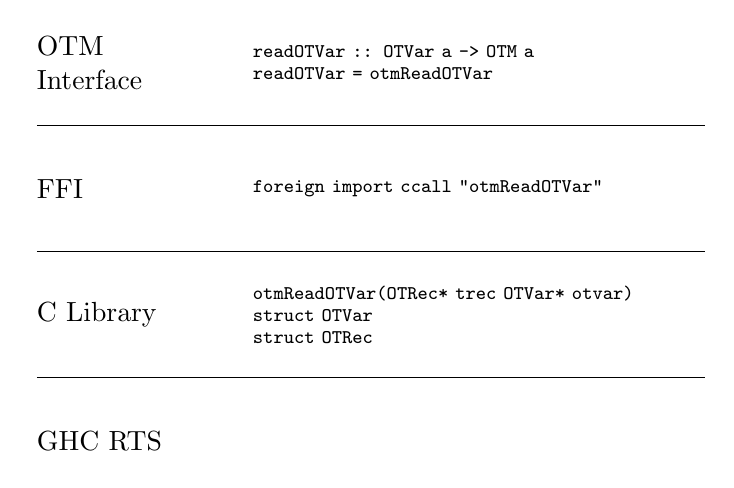
\begin{tikzpicture}[
            lbl/.style={
              text width=2cm,
              %align=center
            },
            lbll/.style={
              font=\scriptsize\ttfamily,
              text width=5cm,
              align=left
            }
        ]
\def\h{8cm}
\def\w{0.7\textwidth}
\foreach \i in {1, 2, 3%, 4
}
    \draw (0, {\i*\h/5}) -- +(\w, 0) {};

\foreach \i/\n in {0/GHC RTS, 1/C Library, 2/FFI, 3/OTM\\Interface%, 4/Haskell \\program
}
    \node[lbl] at (1, {\h/10 + \i*\h/5}) {\n};

\foreach \i/\n in {0/ , 1/otmReadOTVar(OTRec* trec OTVar* otvar)\\struct OTVar\\struct OTRec, 2/foreign import ccall "otmReadOTVar", 3/readOTVar :: OTVar a -> OTM a\\readOTVar = otmReadOTVar%, 4/f :: OTM Int
}
    \node[lbll] at ({0.5*\w+1cm}, {\h/10 + \i*\h/5}) {\n};

\end{tikzpicture}
\end{figure}
\end{frame}

\begin{frame}[fragile]{OTM implementation: read of an open transaction}
Function defined by the C Library:
\begin{verbatim}
HsValue otmReadOTVar(OTRec* otrec, OTVar* otvar) {
    
    otmUnion(otrec, otvar -> trec);

    return otvar -> new_value;
}
\end{verbatim}
\end{frame}

\begin{frame}[fragile]{OTM implementation: merge of transactions}

\begin{itemize}
\item Each transaction records its participants in the transactional log.
\item Merge of transactions are handled with an Union-find data structure.
\item Union-by-rank and path compression heuristics are applied.
\end{itemize}
\note{m make-union-find, di cui n make O(m * a(n))}
\begin{figure}
    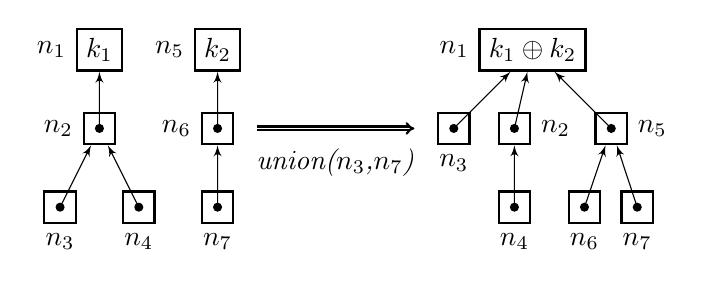
\begin{tikzpicture}
    \node [nodesr, label=left:$n_{1}$] (n1) at (1,2) {$k_{1}$};
    \node [nodesr, label=left:$n_{2}$] (n2) at (1,1) {};
    \node [nodesr, label=below:$n_{3}$] (n3) at (0.5,0) {};
    \node [nodesr, label=below:$n_{4}$] (n4) at (1.5,0) {};
    
    \node [nodesr, label=left:$n_{5}$] (n5) at (2.5,2) {$k_{2}$};
    \node [nodesr, label=left:$n_{6}$] (n6) at (2.5,1) {};
    \node [nodesr, label=below:$n_{7}$] (n7) at (2.5,0) {};
    
    \draw[fill] ($(n2.south)!0.5!(n2.north)$) circle (0.05);
    \draw[fill] ($(n3.south)!0.5!(n3.north)$) circle (0.05);
    \draw[fill] ($(n4.south)!0.5!(n4.north)$) circle (0.05);
    
    \draw[draw, -latex']  ($(n3.south)!0.5!(n3.north)$)  --(n2);
    \draw[draw, -latex']  ($(n4.south)!0.5!(n4.north)$)  --(n2);
    \draw[draw, -latex']  ($(n2.south)!0.5!(n2.north)$)  --(n1);
    
    \draw[fill] ($(n6.south)!0.5!(n6.north)$) circle (0.05);
    \draw[fill] ($(n7.south)!0.5!(n7.north)$) circle (0.05);
    
    \draw[draw, -latex']  ($(n7.south)!0.5!(n7.north)$)  --(n6);
    \draw[draw, -latex']  ($(n6.south)!0.5!(n6.north)$)  --(n5);
    
    %%
    \draw[double, thick, -implies] (3,1) -- node[label=below:\emph{union($n_{3}$,$n_{7}$)}]{} (5,1);
    %%
    
    \node [nodesr, label=left:$n_{1}$] (n1') at (6.5,2) {$k_{1} \oplus k_{2}$};
    \node [nodesr, label=right:$n_{2}$] (n2') at (6.27,1) {};
    \node [nodesr, label=below:$n_{3}$] (n3') at (5.5,1) {};
    \node [nodesr, label=below:$n_{4}$] (n4') at (6.27,0) {};
    
    \node [nodesr, label=right:$n_{5}$] (n5') at (7.5,1) {};
    \node [nodesr, label=below:$n_{6}$] (n6') at (7.16,0) {};
    \node [nodesr, label=below:$n_{7}$] (n7') at (7.83,0) {};
    
    \draw[fill] ($(n2'.south)!0.5!(n2'.north)$) circle (0.05);
    \draw[fill] ($(n3'.south)!0.5!(n3'.north)$) circle (0.05);
    \draw[fill] ($(n4'.south)!0.5!(n4'.north)$) circle (0.05);
    \draw[fill] ($(n5'.south)!0.5!(n5'.north)$) circle (0.05);
    \draw[fill] ($(n6'.south)!0.5!(n6'.north)$) circle (0.05);
    \draw[fill] ($(n7'.south)!0.5!(n7'.north)$) circle (0.05);
    
    \draw[draw, -latex']  ($(n3'.south)!0.5!(n3'.north)$)  --(n1');
    \draw[draw, -latex']  ($(n4'.south)!0.5!(n4'.north)$)  --(n2');
    \draw[draw, -latex']  ($(n2'.south)!0.5!(n2'.north)$)  --(n1');
    
    \draw[draw, -latex']  ($(n6'.south)!0.5!(n6'.north)$)  --(n5');
    \draw[draw, -latex']  ($(n7'.south)!0.5!(n7'.north)$)  --(n5');
    \draw[draw, -latex']  ($(n5'.south)!0.5!(n5'.north)$)  --(n1');
    
    \end{tikzpicture}
    \caption{Merging two transactional log structures.}
    \label{fig:implementation-setrefdiag}
\end{figure}


%The nodes of the data structure are the transactional logs representing transactions.
%Each transaction is represented by a transactional record
%Union-find in which the nodes of the data structure are the transactional records representing a transaction.
\end{frame}

\begin{frame}{OTM implementation: validation of open transactions}
The validation of open transactions is composed by two phases:
\begin{itemize}
\item \emph{voting phase}: each \emph{participant} votes for committing or aborting
\item \emph{agreement phase}: each \emph{participant} commits or aborts depending on the outcome of the previous phase. 
\end{itemize}
\end{frame}

\section{Conclusions}
\begin{frame}{Conclusions}
The OTM model separates isolated transactions from non-isolated ones.
The Haskell implementation is a conservative extension of STM:
\begin{itemize}
\item Semantically \emph{atomically = atomic . isolated}
\item From the user point of view, the libraries have the same interface
\item From the implementation point of view, we provide the same interface of STM against the runtime system
\end{itemize}
Future works:
\begin{itemize}
\item Implement an efficient retry mechanism for transactions
\item Comparison test with Haskell STM
\end{itemize}
\end{frame}

% \begin{frame}{Future works}

% \end{frame}

\end{document}
